\documentclass[11pt]{article}

\usepackage[utf8]{inputenc}
\usepackage[T1]{fontenc}
\usepackage{amsmath,amssymb,amsthm}
\usepackage{mathtools}
\usepackage{graphicx}
\usepackage{booktabs}
\usepackage{hyperref}
\usepackage[margin=1in]{geometry}
\usepackage{enumitem}
\usepackage{xcolor}

\hypersetup{colorlinks=true,linkcolor=blue,citecolor=blue,urlcolor=blue}

\newtheorem{theorem}{Theorem}
\newtheorem{lemma}[theorem]{Lemma}
\newtheorem{corollary}[theorem]{Corollary}
\newtheorem{proposition}[theorem]{Proposition}
\theoremstyle{definition}
\newtheorem{definition}[theorem]{Definition}
\newtheorem{assumption}[theorem]{Assumption}
\newtheorem{remark}[theorem]{Remark}

\newcommand{\node}{\mathsf{n}}
\newcommand{\Nodes}{\mathcal{N}}
\newcommand{\Modules}{\mathcal{M}}
\newcommand{\Chunks}{\mathcal{C}}
\newcommand{\Vals}{\mathcal{V}}
\newcommand{\report}{\mathcal{R}}
\newcommand{\dispatch}{\mathrm{exec}}
\newcommand{\reads}{\rightharpoonup}
\newcommand{\emits}{\rightharpoonup}

\title{A Runtime Without a Program:\\
Execution as Propagation over a Causal Knowledge Graph}

\author{Kundai Farai Sachikonye\\
\small Technical University of Munich\\
\small \texttt{kundai.sachikonye@tum.de}}

\date{\today}

\begin{document}
\maketitle

\begin{abstract}
Conventional operating systems execute a program: an ordered sequence of
instructions whose control flow is, in principle, knowable before the first
instruction runs, and whose termination is reported by an exit code that
signifies success or a class of failure. We describe a runtime that discards
all three of these commitments. The unit of work is not an instruction but a
\emph{node} of a causal knowledge graph, where a node is the convergence of a
subtask and the executable code that realises it. Nodes are produced by
autonomous agents, each module of the system decomposing its problems into
subtasks and publishing them as nodes; every node is readable by every module.
A module consumes the values carried on nodes, transforms them internally, and
emits new values, so that the \emph{trajectory of computation} is not a schedule
but the emergent set of nodes across which information actually propagated. The
operating system carries no semantic responsibility: it executes every code
chunk bundled on a node and judges nothing---it does not compare a result to an
expectation, and therefore cannot fail in the sense an exit code encodes. We
argue this is the correct model for computation organised as \emph{experiment}
rather than \emph{procedure}: results are meaningful only to their consumers,
runs are not expected to be bit-identical, anomalies are recorded rather than
raised, and reproducibility is relocated from the result to the protocol. We
give a formal account of nodes, propagation, run-to-completion semantics, and a
variable-resolution address scheme that lets the same computation be expressed
either coarsely (import a standard setup, touch nothing) or with surgical,
step-by-step control. We validate the core claims---trajectory emergence,
run-to-completion, intended non-determinism, multi-chunk execution, and
resolution control---with a suite of executable Python models.
\end{abstract}

\tableofcontents

\section{Introduction}
\label{sec:intro}

An operating system, in the received sense, is a manager of programs, and a
program is a sequence of instructions. Three assumptions are so deeply
embedded in that sentence that they are rarely stated. First, that the control
flow is a \emph{plan}: even where a program branches on data, the space of
possible sequences is fixed in advance by the code, and the executed sequence is
in principle recoverable. Second, that termination is \emph{adjudicated}: a
process ends with an exit code, and that code is a verdict---zero for success, a
taxonomy of nonzero values for failure---issued by the runtime on the process's
behalf. Third, that execution is \emph{repeatable}: given the same inputs, the
same program is expected to produce the same output, and a divergence is a bug.

These assumptions serve procedural computation well. They serve a different
class of computation badly: computation organised as an \emph{experiment}. A
scientist at a bench does not run a program. They assemble a protocol from
reusable steps, run it to completion, and read the result---and crucially, an
unexpected result does not abort the protocol. It is recorded, and it is the
most valuable thing the run produced, because it is what the eventual
explanation must account for. Nobody expects two runs of a wet-lab assay to be
bit-identical; the measured quantity varies, and the variation is data, not
error. Repeatability, where it exists, is a property of the \emph{protocol and
its provenance}, not of the numbers that come out.

This paper describes a runtime built on the second model. It is the execution
layer of a larger system in which every module solves its problems by
generating autonomous agents, and in which those agents, decomposing problems
into subtasks, are the source of the graph's nodes. We make the following
contributions:

\begin{itemize}[leftmargin=1.4em]
  \item A definition of the \emph{node} as the convergence of a subtask with
  its realising code (Section~\ref{sec:node}), and of the causal knowledge
  graph as the shared, append-structured medium through which modules
  communicate by reading and emitting node values (Section~\ref{sec:graph}).
  \item A semantics for the runtime in which the operating system executes
  \emph{all} code chunks on a node and holds \emph{no} semantic
  responsibility---no comparison to expectation, hence no exit code and no
  halt-on-error (Section~\ref{sec:runtime}).
  \item A characterisation of the \emph{trajectory} of a computation as the
  emergent set of value-bearing nodes, and a proof that this trajectory is not
  knowable in advance and not storable as a plan---only runnable
  (Section~\ref{sec:trajectory}).
  \item A hierarchical \emph{address} scheme giving absolute control at any
  resolution: the same computation is a short address prefix when run from a
  standard setup and a full-depth address when every step is designed by hand
  (Section~\ref{sec:resolution}).
  \item An executable validation of all five claims
  (Section~\ref{sec:validation}).
\end{itemize}

We stress at the outset what the runtime is \emph{not}. It is not a scheduler
that has been made non-deterministic, and its non-determinism is not a
concession to concurrency. The absence of a knowable sequence is structural: the
sequence is a consequence of which modules chose to read which values, a fact
that comes into being only as the run proceeds. Likewise the absence of an exit
code is not a missing feature but a deliberate refusal of the runtime to
arrogate to itself a judgement that belongs only to a consumer.

\section{The node}
\label{sec:node}

\subsection{Agents, modules, and subtasks}

The system is a set of \emph{modules} $\Modules = \{m_1, \dots, m_k\}$. A module
is a competence---a way of solving a class of problems---but it solves nothing
directly. Given a problem, a module generates \emph{agents}, and each agent
decomposes the problem into \emph{subtasks}. This decomposition is the only
source of structure in the system: there is no global problem
decomposition, no master plan, only the union of the decompositions that many
agents, from possibly many modules, happened to produce.

A subtask is not a private matter of the agent that raised it. When an agent's
decomposition arrives at a subtask, that subtask is \emph{published}: it becomes
a node in a graph readable by every module. Two agents---from the same module or
from different modules---that decompose their respective problems and arrive at
the ``same'' subtask converge on a single node. We make ``same'' precise in
Section~\ref{sec:graph}; for now, the picture is that the graph's nodes are
exactly the distinct subtasks that agents have raised, and that convergence is
the norm, not the exception, because different problems share sub-structure.

\subsection{A node is a task fused with its code}

The decisive move is that a node does not merely name a subtask. It carries the
executable code that realises the subtask. In the larger system this code is
written in one or more domain-specific languages (DSLs), and one module,
\emph{Zangalewa}, is dedicated to generating it. When an agent raises a subtask
and a realisation for it is generated, the subtask and its code are fused into
one object.

\begin{definition}[Node]
\label{def:node}
A \emph{node} is a triple
\[
\node \;=\; \bigl(\,\tau,\ \Chunks(\node),\ \Vals(\node)\,\bigr),
\]
where $\tau$ is the identity of a subtask; $\Chunks(\node) = \{c_1, \dots,
c_r\}$ is a finite bag of \emph{code chunks}, each an executable realisation of
$\tau$; and $\Vals(\node)$ is the (time-varying) collection of \emph{values}
the node carries.
\end{definition}

The multiplicity of $\Chunks(\node)$ is essential and is the reason a node is a
\emph{bag} of chunks rather than a single program. A subtask can be realised in
more than one way. An agent may be able to solve the same subtask through two
different modules---so a node may hold, say, a chunk generated for one
module's DSL and, alongside it, a chunk generated for another's. These are not
competing candidates to be selected among. They are co-resident realisations of
one subtask, and, as Section~\ref{sec:runtime} makes precise, the runtime
executes all of them.

\begin{remark}[Convergence, not authorship]
A node is not owned by the agent or module that first raised it. Because the
subtask is what individuates the node, and because many agents converge on the
same subtask, a node accretes chunks and values from every agent that reaches
it. The node is a \emph{meeting point}, and its content is the union of what
converged there. This is why the node's values are ``material'' for the whole
system rather than the private state of one computation.
\end{remark}

\subsection{Values are the medium of exchange}

The third component, $\Vals(\node)$, is what makes the graph a communication
medium and not merely a catalogue of code. A value is any piece of information a
module cares to attach to a node: a measured quantity, a derived record, a
finding, a partial result. The contract between modules is stated entirely in
terms of values:

\begin{quote}
Every module \emph{emits} values onto nodes and \emph{reads} values from nodes.
A module reads the values on a node, makes internal changes on the strength of
what it read, and emits new values---possibly onto the same node, possibly onto
others.
\end{quote}

No module reads another module's internal state, and no module is required to
understand another module's code chunks. The only shared surface is
$\Vals$. This is what we mean by saying the runtime has no semantic
responsibility (Section~\ref{sec:runtime}): the runtime moves values by
executing chunks, and what a value \emph{means} is entirely a matter for the
module that reads it.

\section{The causal knowledge graph}
\label{sec:graph}

\subsection{Nodes, and the edges the runtime does not store}

Let $\Nodes$ be the set of all nodes. One might expect a computation to be
specified by a graph $G = (\Nodes, E)$ with a fixed edge set $E$ encoding ``node
$u$ feeds node $v$.'' It is not. An edge in this system is a \emph{causal}
relation---``a value emitted at $u$ was read at $v$''---and such a relation
exists only once the reading has happened.

\begin{proposition}[Edges are generated, not stored]
\label{prop:no-edges}
The causal relation on $\Nodes$ is not a fixed attribute of the graph. An edge
$u \to v$ obtains in a run if and only if, in that run, a value emitted at $u$
was read by a module that then emitted at $v$. Consequently the edge set is a
\emph{product} of a run, not an \emph{input} to it, and two runs over the same
$\Nodes$ may induce different edge sets.
\end{proposition}

\noindent This is the first sense in which the graph is ``causal'': its edges are
records of causation that occurred, not declarations of dependency to be
scheduled. The nodes are the durable objects; the edges are ephemeral.

\subsection{Identity and convergence}

We said two agents that arrive at the ``same'' subtask converge on one node.
Formally, identity is carried by $\tau$: nodes are individuated by their subtask
identity, and everything else about a node---its chunks, its values---accretes
onto that identity. A subtask at rest is a name; a subtask in motion is a
carrier of values. The two are the same object, seen once as an entry in a
catalogue of what \emph{can} be computed and once as a live participant in what
\emph{is being} computed.

\begin{definition}[Convergence]
\label{def:convergence}
Two subtask realisations \emph{converge} when they share subtask identity
$\tau$. Convergence merges their chunk bags and unifies their value collections
onto the single node bearing $\tau$. The graph therefore grows by convergence:
raising a subtask that already exists adds chunks and values to an existing
node rather than creating a new one.
\end{definition}

\subsection{The four things a module does to a node}

A module interacts with the graph through a small, closed vocabulary. It can
\emph{identify} a node (find the node bearing a subtask), \emph{read} its
values, \emph{transform} internally, and \emph{emit} new values. There is no
fifth verb: a module cannot, for instance, ask the graph whether a value is
\emph{correct}, because correctness is not a property the graph represents. The
graph stores what was emitted, not what should have been. This closure is what
forces adjudication out of the runtime and into the consumers, and it is the
structural root of the no-exit-code result of Section~\ref{sec:runtime}.

\section{The runtime}
\label{sec:runtime}

\subsection{Execution is the only responsibility}

\begin{definition}[Node execution]
\label{def:exec}
To \emph{execute} a node $\node$ is to run every chunk in its bag:
\[
\dispatch(\node) \;=\; \bigl\langle\, \dispatch(c) : c \in \Chunks(\node)
\,\bigr\rangle,
\]
each chunk producing whatever value deltas it produces, all of which are emitted
onto the graph. The runtime performs $\dispatch(\node)$ and nothing else. It
does not select among chunks; it does not order the graph; it does not inspect
the values that result.
\end{definition}

The runtime is, in this precise sense, \emph{semantically inert}. It is a device
for turning nodes into value emissions by running their code. Two consequences
follow, and they are the heart of the design.

\subsection{No exit code}

\begin{theorem}[No exit code]
\label{thm:no-exit}
The runtime cannot emit an exit code, because an exit code presupposes a
comparison the runtime is structurally unable to make.
\end{theorem}

\begin{proof}
An exit code is a verdict: success versus a class of failure. To issue it, the
issuer must compare an achieved state to an expected one. The runtime's entire
interface with meaning is the value collection $\Vals$, and---by the closure of
Section~\ref{sec:graph}---the graph has no verb for ``expected'' and stores no
expectation against which an achieved value could be measured. The runtime
therefore has no expected state to compare against, and no comparison operator
in its vocabulary. Whatever a chunk emits is simply emitted; there is no state
in which the runtime holds a belief about what \emph{should} have been emitted.
Hence there is no quantity the runtime could compute that would have the meaning
of an exit code. Adjudication is possible only downstream, in a consumer that
holds an expectation of its own; and a consumer's judgement is that consumer's,
not the runtime's.
\end{proof}

\subsection{Run to completion}

\begin{corollary}[Run to completion]
\label{cor:completion}
The runtime does not halt on an unexpected result or an error emitted by a
chunk. It runs each node's chunks and moves on; anomalous emissions are recorded
as values like any other.
\end{corollary}

\begin{proof}
By Theorem~\ref{thm:no-exit} the runtime has no notion of ``unexpected,'' so
there is no event of type ``unexpected result'' for it to halt on. A chunk that
throws produces a value---an error record---which is emitted onto the graph
exactly as a numeric result would be. Nothing in $\dispatch(\node)$ branches on
the \emph{content} of an emission, so the presence of an error value cannot
alter control flow. The run proceeds until there are no more nodes carrying
unpropagated values.
\end{proof}

This is the bench semantics stated formally. In a wet-lab protocol an
unexpected reading does not abort the assay; it is written in the notebook and
becomes the thing the analysis must explain. Here, identically, an anomaly is a
first-class value on a node, available to any module that reads it and to the
final report. The report---not an exit code---is the runtime's output, and the
report's job is to \emph{account for} what happened, anomalies included.

\begin{remark}[Where errors are handled]
Corollary~\ref{cor:completion} does not say errors are ignored. It says they are
not handled \emph{by the runtime}. A module that reads an error value may do
anything it likes with it---retry through a different chunk, emit a diagnostic
value, raise a finding for the report. That is a module's semantic prerogative.
The runtime's refusal to act on error content is what keeps the semantics in the
modules where it belongs.
\end{remark}

\section{The trajectory}
\label{sec:trajectory}

\subsection{Definition}

\begin{definition}[Trajectory]
\label{def:trajectory}
The \emph{trajectory} of a run is the set of nodes that carried propagated
information during that run---the nodes at which some module read a value and,
on the strength of it, emitted a value that another module later read. Formally
it is the vertex set of the induced causal edge relation of
Proposition~\ref{prop:no-edges}, together with the node values as they stood
when they were read.
\end{definition}

The trajectory is what a procedural system would call the ``execution trace,''
but the analogy is misleading, because a trace is a record of a sequence that
was determined by a program. Here there is no program to determine a sequence.
The trajectory is the sequence, and it is constituted by the reads and emits
that actually occurred.

\subsection{The trajectory is not a plan}

\begin{theorem}[Trajectory emergence]
\label{thm:emergence}
The trajectory of a run is not knowable before the run and is not storable as a
schedule. It can only be produced by running.
\end{theorem}

\begin{proof}
Membership of a node in the trajectory depends on whether some module read a
value there and emitted onward. Whether a module reads a given value is a
decision the module makes on the strength of values it has \emph{already} read
in this run (Section~\ref{sec:node}). Thus the trajectory at step $t$ is a
function of the values present at step $t$, which are the emissions of steps
$< t$, which depend on the trajectory up to $t{-}1$. The relation is a fixed
point of a map that takes a partial trajectory to its own extension. Because the
map's action at each step consults run-produced values---not any datum available
before the run---no evaluation of the map is possible without executing the
steps it depends on. A stored schedule would have to name the sequence of nodes
in advance; but the sequence is the fixed point just described, and the fixed
point is defined by the run. Hence the trajectory is runnable but not
pre-computable and not storable as a plan.
\end{proof}

\begin{corollary}
The set of nodes---the ``what can be computed''---is durable and can be
catalogued, imported, and frozen. The trajectory---the ``what was
computed''---cannot. Reproducibility must therefore attach to the former.
\end{corollary}

\noindent We return to this corollary in Section~\ref{sec:repro}: it is why
repeatability in this system is a property of the setup and its provenance, never
of the results.

\subsection{Figure: trajectory as emergent, not scheduled}

\begin{figure*}[t]
  \centering
  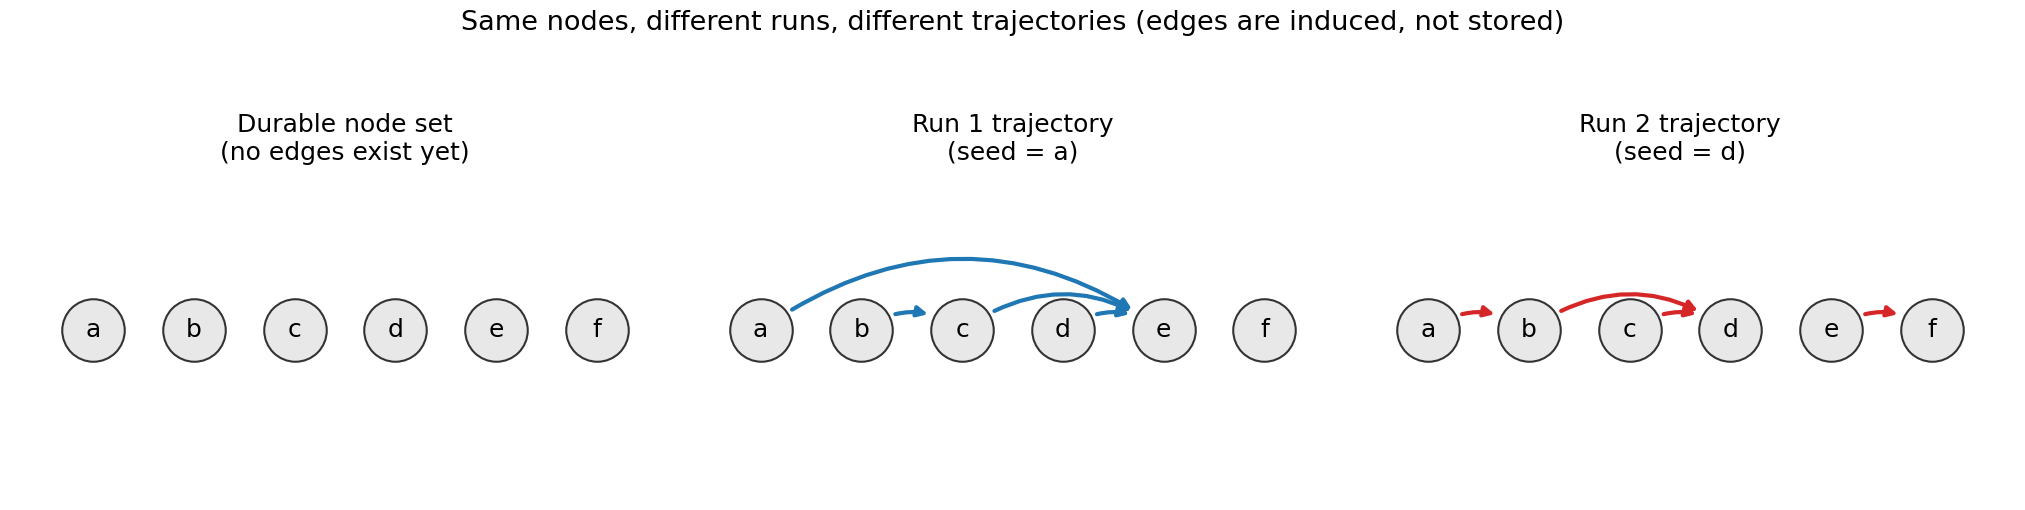
\includegraphics[width=0.9\textwidth]{figures/trajectory_emergence.png}
  \caption{\textbf{The trajectory is a product of the run, not an input to it.}
  Left: the durable node set---the subtasks that can be computed---with no edges,
  because edges do not exist until a run induces them
  (Proposition~\ref{prop:no-edges}). Centre and right: two runs over the
  \emph{same} node set induce different causal edge relations and therefore
  different trajectories (highlighted), because which values were read differed
  between runs. No schedule over the node set could have named either trajectory
  in advance (Theorem~\ref{thm:emergence}). Panel generated by
  \texttt{validation/trajectory\_emergence.py}.}
  \label{fig:emergence}
\end{figure*}

\section{Resolution: absolute control at any depth}
\label{sec:resolution}

\subsection{The problem of control}

A benchtop scientist can, if they wish, design every step of an analysis by
hand---every reagent, every incubation, every wash. Usually they do not: they
import a standard protocol and run it untouched. The same apparatus must serve
both the coarse user, who wants to import a standard setup and change nothing,
and the surgical user, who wants to account for every single step. Crucially,
these are not two systems. They are one computation described at two
resolutions.

\subsection{Hierarchical addresses}

We make ``resolution'' precise with an address scheme. Every element of the
system---a module, a node, a chunk within a node, a value within a
chunk---receives a hierarchical address, a finite sequence of components from
coarsest to finest:
\[
a \;=\; \langle a_1, a_2, \dots, a_k \rangle,
\qquad k = \operatorname{depth}(a).
\]
A short address names a coarse region of the computation---a whole standard
setup, say. A long address reaches through that region to a single step inside
it. The two describe the \emph{same object} at different depths: the standard
setup \emph{is} the surgical design, addressed less finely.

\begin{definition}[Resolution]
\label{def:resolution}
The \emph{resolution} at which a user works is the depth $k$ at which they
address the computation. A \emph{coarse} run addresses a short prefix---it names
a standard setup and touches nothing beneath it. A \emph{surgical} run addresses
at full depth---it names, and may redesign, every step. Both act on the same
underlying nodes; they differ only in how deeply the user reaches.
\end{definition}

\begin{proposition}[Prefix containment]
\label{prop:prefix}
If address $a$ is a prefix of address $b$, then the object named by $b$ lies
within the region named by $a$. Editing at depth $k$ leaves every object whose
address does not share the length-$k$ prefix untouched, and reveals for editing
every object beneath that prefix. Coarse and surgical control are thus the
\emph{same} address space traversed to different depths, and a user may descend
to exactly the depth a given step requires and no further.
\end{proposition}

\noindent The consequence is the design goal stated plainly: the system gives
absolute control over any element of the computation, exercised only where the
user chooses to exercise it. Different experts may work at full depth in
different regions---one module's steps designed surgically by a specialist,
another's imported as a standard---and the whole remains one addressable object.
No conventional operating system offers this, because in a conventional system
the ``standard setup'' (a library call) and the ``surgical design'' (the
library's source) are different artefacts at different times, not one object at
two depths of a single live address space.

\subsection{Importing a standard setup}

Because the node set is durable (Theorem~\ref{thm:emergence}, corollary), a
region of it can be \emph{frozen} and \emph{imported}. Importing a standard setup
is addressing a subtree by its short prefix and accepting everything beneath
without descent. The import mechanism is subtree selection: a standard setup is a
named subtree of the node catalogue; importing it grafts that subtree, chunks and
frozen values and all, into the user's computation, to be run as-is.

\begin{figure*}[t]
  \centering
  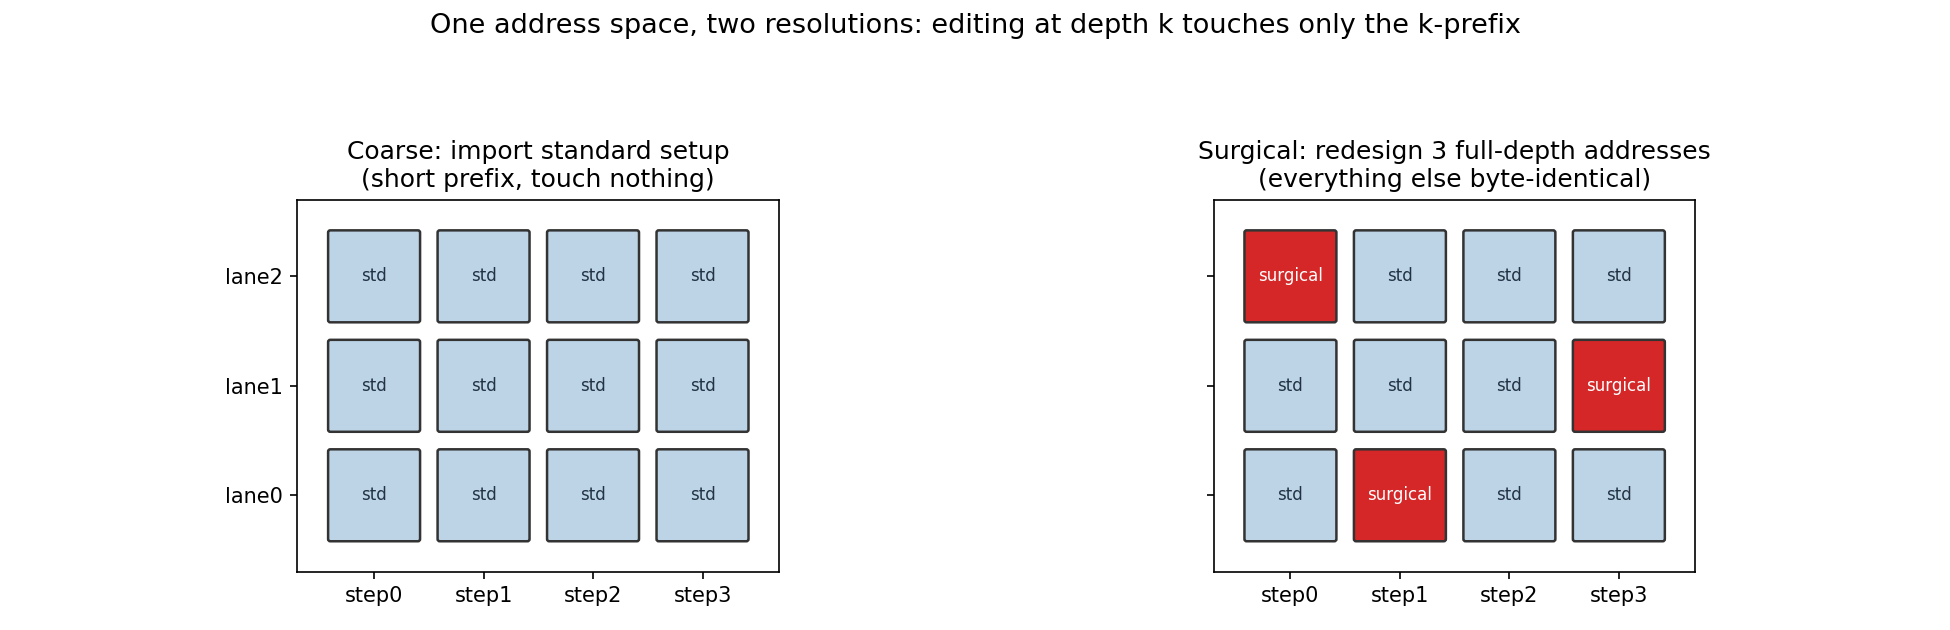
\includegraphics[width=0.92\textwidth]{figures/resolution_control.png}
  \caption{\textbf{One computation at two resolutions.} The same node subtree is
  shown addressed coarsely (top: a single short-prefix address names an imported
  standard setup, run untouched) and surgically (bottom: full-depth addresses
  reach individual steps, three of which are redesigned by hand). Editing at
  depth $k$ touches only objects sharing the length-$k$ prefix
  (Proposition~\ref{prop:prefix}); everything else is byte-identical between the
  two runs. Panel generated by \texttt{validation/resolution\_control.py}.}
  \label{fig:resolution}
\end{figure*}

\section{Reproducibility relocated}
\label{sec:repro}

The final consequence of the design concerns what it means for a computation to
be reproducible. In a procedural system, reproducibility is a property of
results: the same program on the same input yields the same output, and a
divergence is a defect. Here that expectation is abandoned deliberately.

\begin{proposition}[Intended non-determinism]
\label{prop:nondeterminism}
Two runs of the same computation are not expected to produce identical values,
for two independent reasons. First, chunks may realise measurements or other
processes whose outputs vary between runs, exactly as a physical measurement
varies. Second, by Theorem~\ref{thm:emergence} the trajectory itself is
run-constituted, so even value-preserving chunks may be read in a different
order and induce a different causal edge relation. Non-determinism is therefore
structural, not incidental, and is not treated as error.
\end{proposition}

If results are not expected to repeat, what does reproducibility mean? It
relocates to the \emph{protocol and its provenance}. What repeats is the setup:
the node subtree that was imported, the chunks that were bundled, the addresses
at which the user reached in to redesign. A run records this provenance in its
report, and another party can reproduce the run by importing the same standard
setups and reaching to the same addresses---and then expect, not the same
numbers, but a run of the same protocol, whose differing numbers are themselves
data. This is precisely the sense in which a wet-lab result is reproducible: not
that the readings coincide, but that the protocol can be re-enacted and its
readings compared.

\begin{figure*}[t]
  \centering
  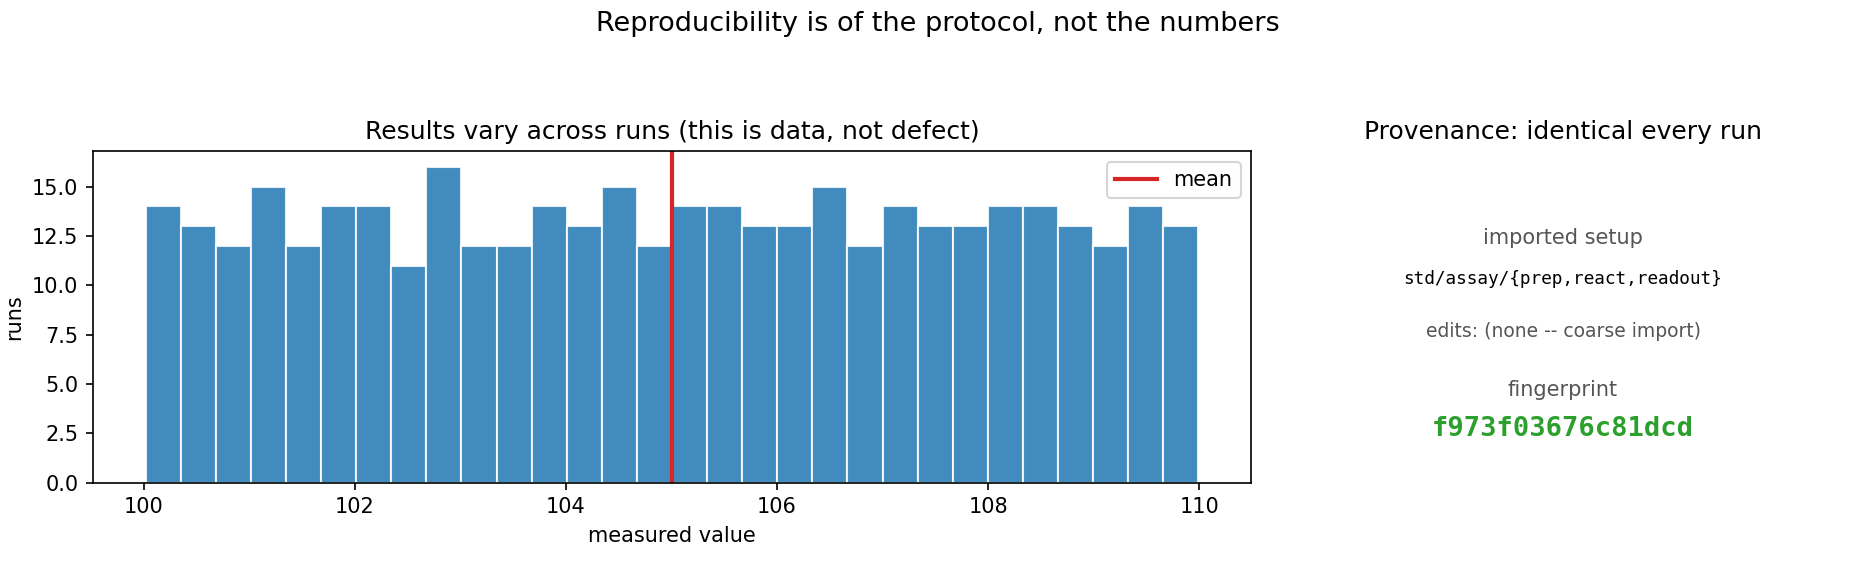
\includegraphics[width=0.9\textwidth]{figures/nondeterminism_provenance.png}
  \caption{\textbf{Reproducibility attaches to the protocol, not the results.}
  Repeated runs of one imported standard setup produce a spread of result values
  (left, histogram) while sharing an identical provenance fingerprint (right:
  the imported subtree, chunk bag, and edit addresses are byte-identical across
  all runs). The variation on the left is data, not defect
  (Proposition~\ref{prop:nondeterminism}); the invariance on the right is what
  reproducibility means here. Panel generated by
  \texttt{validation/nondeterminism\_provenance.py}.}
  \label{fig:nondeterminism}
\end{figure*}

\section{Validation}
\label{sec:validation}

We validate the five load-bearing claims with executable Python models. Each is
a self-contained simulation of the runtime's mechanics---nodes as
task/chunk/value bundles, modules as read/transform/emit agents, the runtime as
a chunk executor that judges nothing---instrumented to test one claim. The
scripts live under \texttt{validation/} and write the figure panels into
\texttt{figures/}.

\begin{table}[h]
  \centering
  \begin{tabular}{@{}p{0.30\textwidth}p{0.62\textwidth}@{}}
    \toprule
    \textbf{Claim} & \textbf{What the validator demonstrates} \\
    \midrule
    Trajectory emergence
    (Thm.~\ref{thm:emergence}) &
    Two runs over an identical node set induce different causal edge relations;
    no static schedule reproduces either. \\[0.4em]
    No exit code / run to completion
    (Thm.~\ref{thm:no-exit}, Cor.~\ref{cor:completion}) &
    A chunk that raises does not halt the run; the error becomes a recorded
    value and the runtime emits no verdict. \\[0.4em]
    Multi-chunk execution
    (Def.~\ref{def:exec}) &
    A node bearing two chunks from different modules runs both; both value
    deltas appear on the graph. \\[0.4em]
    Intended non-determinism
    (Prop.~\ref{prop:nondeterminism}) &
    Repeated runs of one setup spread over result values while sharing one
    provenance fingerprint. \\[0.4em]
    Resolution control
    (Prop.~\ref{prop:prefix}) &
    Editing at depth $k$ changes only objects under the length-$k$ prefix; a
    coarse import and a surgical redesign are the same address space. \\
    \bottomrule
  \end{tabular}
  \caption{The validation suite. Each row is one script under
  \texttt{validation/}.}
  \label{tab:validation}
\end{table}

The validators are written against the same runtime shape used in the production
system: a module exposes an identity and an \texttt{execute} step that returns a
value delta together with a completion flag, a dispatcher runs a node's chunks
and appends an audit record without inspecting the returned values, and the only
run output is a report assembled from emitted values. The simulations are
faithful to that shape so that a passing validator is evidence about the runtime,
not about an unrelated toy.

\section{Related notions}
\label{sec:related}

The runtime touches several established bodies of work while committing to none
of them wholesale. Its read/transform/emit modules over a shared node medium
resemble dataflow and actor models of computation~\cite{kahn1974semantics,
lee1995dataflow, hewitt1973actor, agha1986actors}, but it departs from them in
refusing a fixed dependency graph: edges are run-induced
(Proposition~\ref{prop:no-edges}), not declared. Its treatment of the graph as a
queryable store of what was emitted, with a closed retrieval
vocabulary, is in the spirit of knowledge-graph and query-language
semantics~\cite{hogan2021knowledge, perez2009sparql}, but it deliberately omits
any predicate of correctness, which is what forces adjudication out of the store.
Its relocation of reproducibility from results to provenance draws on the
provenance and workflow literature~\cite{moreau2013prov, davidson2008provenance},
and on the broader discussion of reproducibility in computational
science~\cite{peng2011reproducible, sandve2013reproducible}. Its embrace of
run-to-completion over halt-on-error is the computational analogue of the
experimental stance that an anomaly is recorded and explained rather than
raised. Finally, the variable-resolution address scheme
(Section~\ref{sec:resolution}) is a hierarchical namespace in the tradition of
tries and prefix structures~\cite{fredkin1960trie}, used here not for lookup but
for control: prefix depth \emph{is} the resolution of user intervention.

\section{Conclusion}
\label{sec:conclusion}

We have described a runtime that executes a causal knowledge graph rather than a
program. Its nodes are subtasks fused with their realising code, produced by the
agents that modules generate; its modules communicate solely by reading and
emitting values on those nodes; and its operating system executes every chunk on
a node while judging nothing. From that semantic inertia three properties follow
that no procedural runtime has: there is no exit code, because the runtime holds
no expectation to compare against; there is no knowable schedule, because the
trajectory is constituted by the reads and emits of the run itself; and there is
no expectation of identical results, because non-determinism is structural and
reproducibility has been relocated to the protocol. A hierarchical address scheme
then gives absolute control at any resolution, so that the same computation is a
short prefix when imported as a standard setup and a full-depth address when
designed surgically---one object, reachable to whatever depth a step demands.
The result is an execution model for computation-as-experiment: run to
completion, record the anomaly, explain it in the report, and reproduce the
protocol rather than the numbers.

\bibliographystyle{plain}
\bibliography{references}

\end{document}
